\chapter{Sentiment analysis and personality trait detection}
\label{ch:sentiment_analysis}
\textbf{John Culnan, Adarsh Pyarelal}
\section{Introduction}

Personality trait detection, sentiment analysis, and related measures of
personal characteristics like emotion recognition are all frequently
used to characterize an object of study. As such, they provide an AI agent with
information about the background and states of individuals at any given time,
which may be used to allow the agent to interact with individuals in a manner
appropriate to their current state. Because understanding the personalities and
emotional states of other individuals is a key feature of collaboration among
people, it is a critical component of the identification of the overall mental
states of others as required for a machine theory of mind
\cite{Rabinowitz.ea:2018}. Providing an AI agent with this capability will
likewise help inform a machine theory of teamwork by allowing the AI agent to
incorporate a wider range of key information in performing its own role.

Our speech-based system of personal characteristic identification currently
includes predictions for emotion and dominant personality trait, and will be
extended during Study 3 to include both a sentiment task and an emotional intensity
task. The emotion task attempts to identify the emotion of each utterance from six
emotions (anger, disgust, fear, joy, sadness, surprise) and a neutral option. The
dominant personality trait task identifies which personality trait is dominant for
a person from among the Big Five personality traits (agreeableness, conscientiousness,
extroversion, neuroticism/emotional stability, and openness to experience). The
sentiment task seeks to identify whether the speaker shows positive, negative, or
neutral sentiment during an utterance. Finally, the emotional intensity task aims to
categorize emotional utterances as either showing a strong or weak level of emotion.

There are no existing state of the art (SOTA) models for the Study 3 dataset, as the
data collection has not been completed yet; however, SOTA models
exist for related datasets and tasks, some of which are incorporated into our
model as task-specific training data. For the Multimodal Emotion Lines Dataset (MELD)
\cite{Poria.ea:2019}, which consists of data from the television show Friends that
has been annotated for both sentiment and emotion, the
SOTA model is TODKAT \cite{Zhu.ea:2021}, which uses context-aware
text and audio transformer-based models for the emotion recognition task. The
First Impressions V2 dataset \cite{Ponce-Lopez.ea:2016}, consisting of the Big
Five personality trait classification for YouTube clips, was originally created
for use as a regression task of identifying the extent to which each speaker
has each personality trait; for the task of classifying the dominant personality
trait, the SOTA model is \citet{Culnan.ea:2021}. The Multimodal Opinion-Level
Sentiment Intensity (MOSI) dataset \cite{Zadeh.ea:2016} consists of single
speakers in YouTube clips providing opinions that are rated from highly
negative to highly positive. The current SOTA model for MOSI is
TupleInfoNCE \cite{Liu.ea:2021}, which uses contrastive learning on augmented
data.

One major limitation of current SOTA approaches is that the data on which they
are trained is not varied in source; typically, each task is trained
separately, so that when two or more tasks have similar or identical label
spaces, the model is retrained for each new task. The data within a given task
generally includes speakers with the same native language.  Multi-party data
furthermore frequently come from scripted sources, such as the television show
Friends \cite{Poria.ea:2019, Zhu.ea:2021}), and single party data from YouTube
\cite{Zadeh.ea:2016, Ponce-Lopez.ea:2016}). Finally, these SOTA models are
created around datasets that rely on accurate, hand-crafted transcriptions of
the audio data, without considering imperfections in the transcriptions. We
approach this challenge by examining the Study 3 data through multitask neural
networks that make use of both existing corpora as pre-training data as well as
the Study 3 data to perform the same tasks in a new domain. We further seek to
improve performance by giving special consideration to the imperfection of
automatic ASR transcriptions used with the Study 3 data.


\section{Approach}

Our approach includes a hard parameter sharing multitask model pre-trained on
tasks for sentiment \citep{Zadeh.ea:2016}), emotion \citep{Poria.ea:2019}),
personality trait \citep{Ponce-Lopez.ea:2016}),
and emotional intensity \citep{Livingstone.ea:2018}), then trained on data from
Study 3. Like \citet{Liu.ea:2021}, our model will make use of augmented data to
allow for more balanced classes in each dataset of interest.  Acoustic and text
data will be fed into the model separately, with text data masked to handle
noise created by automatic transcription. These text transcriptions will be
paired in an ensemble with predictions made by a trained wav2vec model
\citep{Schneider.ea:2019}, which will allow for further boosting of text
modality accuracy. Acoustic and text data will subsequently be concatenated
prior to making predictions about the classes for each utterance-level data
point. A schematic representing our approach is shown in
\autoref{fig:sentiment_model_schematics}.

\begin{figure}
    \begin{sidecaption}{%
        Schematic representation of our multitask model
    for classifying speech according to speaker's dominant personality trait,
    emotion, emotional intensity, and sentiment. The model makes use of both
    speech-based audio input and content-based text input. During Study 3,
    text representations will be augmented with output of a wav2vec system
    providing further information about the way the words were produced.
    Speech- and text-based modalities are fed through neural layers separately,
    then concatenated and fed through an additional neural layer before a final
    task-specific layer is used to make predictions on each of the four tasks
    simultaneously. }[fig:sentiment_model_schematics]
    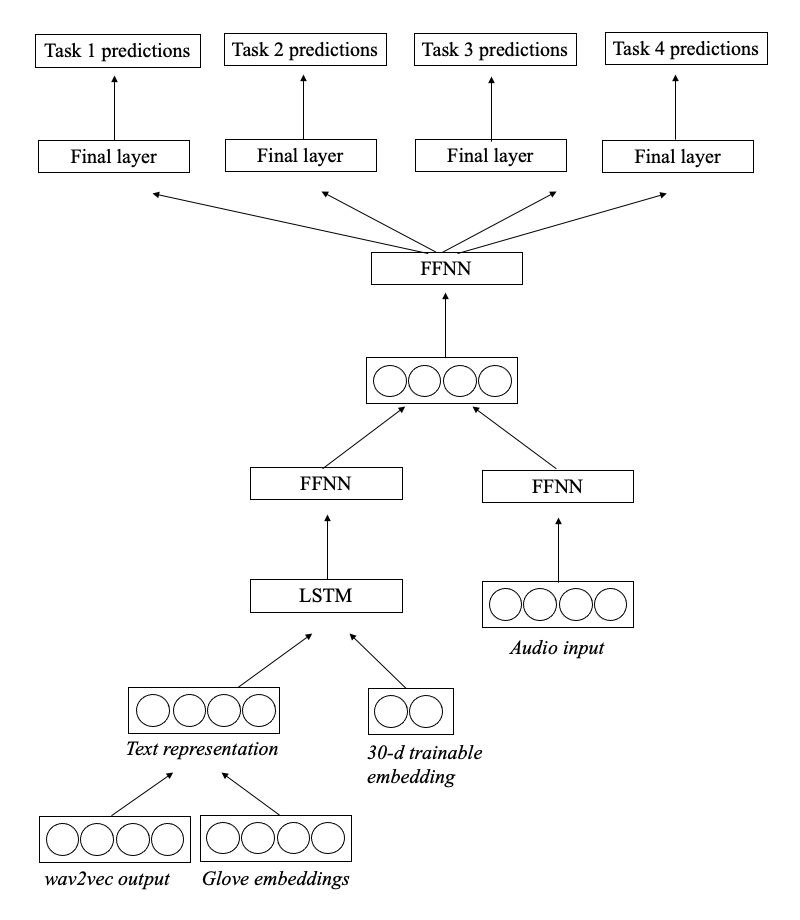
\includegraphics[width=\textwidth]{../images/sentiment_schematics_study3.png}
    \end{sidecaption}
\end{figure}

The experiments we propose to run with our model are based on an initial
analysis of two versions of our existing model's results on a subset of the
Study 3 Spiral 3 pilot data. The results of this initial analysis are shown in
\autoref{tab:spiral3_analysis} In this initial analysis, we compared models
trained with and without information about the distribution of class labels in
the training (non-ASIST) datasets (i.e., with and without class weights).  For
the Study 3 Spiral 3 pilot data, the model trained with class weights achieved
an F1 score of 58.78 for emotion recognition (comparable to the score achieved
on the test partition of MELD). However, the model trained without class
weights performed better, reaching an F1 score of 72.64.

\begin{table}
    \small
    \centering
    \begin{tabular}{lcc}
        \toprule
        Model type & Emotion & Personality Trait \\
        \midrule
        Class weights & 58.78 & 21.58 \\
        No class weights & 72.64 & 37.65 \\
        \bottomrule
    \end{tabular}
    \caption{%
        Performance of trained models with and without class weights on
        emotion and dominant personality trait tasks. Numbers shown are F1 scores
        for emotion and personality trait. Gold labels for personality traits are
        determined using results of the Ten Item Personality Inventory survey,
        while gold labels for emotion were created through annotation of data
        points by two researchers.
    }
    \label{tab:spiral3_analysis}
\end{table}

For dominant personality trait identification, the results similarly showed
improvement when the model did not include class weights (F1 of 21.58 for Study
3 Spiral 3 data with class weights, F1 of 37.65 for this data without class
weights). These scores were calculated by using annotations for emotion and
sentiment by two researchers on our team as gold labels, as well as Ten Item
Personality Inventory (TIPI) survey results for personality trait
identification gold labels.

Results of both tasks may not have been representative of the true performance
of the model, as the Spiral 3 data used confederates (i.e., members of the
research team) rather than naive participants; it is possible these
participants did not respond to the TIPI in the same way that naive
participants would have, and this group of pilot participants may have been
calmer or more neutral in their speech due to their previous experience with
the missions and data collection procedure. To determine whether this is the
case, data from Study 3 will need to be annotated, with results from a portion
of Study 3 participants compared to the results of Spiral 3
participants\footnote{While data was collected from a set of naive participants
prior to the drafting of this preregistration, this data did not include the
necessary vocalic features for our analysis, due to technical issues. We expect
that the rest of the Study 3 data will contain these features.}.

Furthermore, while the model trained without use of information on the distribution
of gold labels in the training datasets outperformed the model trained with this
information, the model without distributional information did not make predictions
for all possible emotions and traits. In order to rectify this and attempt to
further improve the quality of model predictions, the distribution of data points
across all emotions and traits in the ASIST-specific data rather than pretraining
datasets will be incorporated into this model, as such information may provide an
additional boost to model performance.

The Study 3 data that will be incorporated into our models are:

\begin{enumerate}
    \item the
pre-experiment TIPI survey \\
(Participant\_CognitiveTenItemPersonalityInventory\_Survey\_PreExperiment)
    \item the
text output of the ASR system \\
(MinecraftEntity\_Observation\_Asr\_Speechanalyzer)
    \item the audio data and the
acoustic features extracted from this audio signal
(MinecraftEntity\_Observation\_Audio\_Speechanalyzer)
\end{enumerate}

In addition to this previously collected data, new
utterance-level annotations will be collected for sentiment, emotion, and
emotional intensity. The text output of the ASR system and the acoustic features
extracted from the audio signals will be used as input data in the model,
while the TIPI and new utterance-level annotations will be used as gold labels
to evaluate the performance of our model.

\section{Evaluation}

System evaluation will consist of examinations of the network's ability to make
correct predictions about sentiment, emotion, and personality traits using F1
scores calculated by comparing network predictions with survey responses and
human-annotated data as described above. To provide comparable scores to
existing models for these tasks, average F1 scores will be used, calculated as
the weighted average of the F1 score for each class in the task.  Bootstrap
resampling \cite{kohavi1995study} will be used to provide statistical
comparisons among models created for these tasks, enabling the identification
of the best model.

While F1 calculations provide information on the overall success rate of our
models, they are limited in their ability to identify areas of weakness. To
further evaluate the ability of each of our models to perform under the different
conditions available, a subset of incorrect data points will be examined.
Patterns of errors that demonstrate model weaknesses with a particular type of
data (such as difficulty in correctly identifying neutral sentiment in male
voices) will be used to inform further iterations of network updates.

\section{Results}

We were not able to add the results for this analysis in time for the deadline.
We expect to update this document soon with the results.
